\documentclass[aspectratio=169]{beamer}
\usepackage{graphicx}
\usepackage{tikz}
\usepackage{fontawesome5}
\usepackage{hyperref}

% Theme
\usetheme{Madrid}
\usecolortheme{default}

% Custom colors - TRACE Brand
\definecolor{tracedark}{RGB}{3,4,94}
\definecolor{traceblue}{RGB}{0,119,182}
\definecolor{tracecyan}{RGB}{0,180,216}
\definecolor{tracelight}{RGB}{144,224,239}

\setbeamercolor{structure}{fg=tracedark}
\setbeamercolor{palette primary}{bg=tracedark,fg=white}
\setbeamercolor{palette secondary}{bg=traceblue,fg=white}
\setbeamercolor{palette tertiary}{bg=tracecyan,fg=white}
\setbeamercolor{frametitle}{bg=tracedark,fg=white}

% Title Information
\title{\textbf{TRACE}}
\subtitle{Transparent Results \& Academic Compliance Engine}
\author{Team TRACE}
\institute{University of Hyderabad}
\date{\today}

\begin{document}

% ============================================
% SLIDE 1: Title Slide
% ============================================
\begin{frame}
\titlepage
\begin{center}
\includegraphics[width=0.15\textwidth]{logo.jpeg}\\
\vspace{0.3cm}
\textcolor{traceblue}{\large AI-Powered Academic Management System}
\end{center}
\end{frame}

% ============================================
% SLIDE 2: Problem Statement
% ============================================
\begin{frame}{The Problem We're Solving}
\frametitle{Critical Challenges in Academic Management}

\begin{center}
\textcolor{red}{\Large\textbf{The Grading Crisis}}
\end{center}

\vspace{0.3cm}

\begin{columns}
\column{0.5\textwidth}
\textbf{\large The Numbers:}
\begin{itemize}
    \item Faculty spend \textcolor{red}{\textbf{15 minutes}} per assignment
    \item With 90 students = \textcolor{red}{\textbf{22.5 hours/week}} grading
    \item Students wait \textcolor{red}{\textbf{2+ weeks}} for feedback
    \item \textcolor{red}{\textbf{30\%}} of students fail without early warning
    \item Inconsistent grading across \textcolor{red}{\textbf{multiple evaluators}}
\end{itemize}

\vspace{0.3cm}
\textbf{\large The Impact:}
\begin{itemize}
    \item \textbf{Faculty:} No time for teaching/research
    \item \textbf{Students:} Late feedback = poor learning
    \item \textbf{Admins:} Can't identify at-risk students early
    \item \textbf{Institution:} Higher dropout rates
\end{itemize}

\column{0.5\textwidth}
\begin{center}
\textbf{Faculty Time Distribution}\\
\vspace{0.3cm}
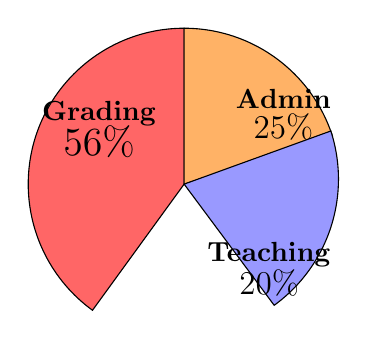
\begin{tikzpicture}[scale=0.9]
% Pie chart
\draw[fill=red!60] (0,0) -- (0,2.2) arc (90:234:2.2) -- cycle;
\node at (-1.2,1) {\textbf{Grading}};
\node at (-1.2,0.6) {\Large 56\%};

\draw[fill=orange!60] (0,0) -- (0,2.2) arc (90:18:2.2) -- cycle;
\node at (1.4,1.2) {\textbf{Admin}};
\node at (1.4,0.8) {\large 25\%};

\draw[fill=blue!40] (0,0) -- (2.07,0.75) arc (18:-54:2.2) -- cycle;
\node at (1.2,-1) {\textbf{Teaching}};
\node at (1.2,-1.4) {\large 20\%};
\end{tikzpicture}

\vspace{0.5cm}
\colorbox{red!30}{\parbox{0.9\textwidth}{
\centering
\textbf{Problem: Faculty spend more time grading than teaching!}
}}
\end{center}
\end{columns}

\vspace{0.3cm}
\begin{center}
\textcolor{tracedark}{\textbf{TRACE solves this with AI automation + predictive analytics}}
\end{center}
\end{frame}

% ============================================
% SLIDE 3: Solution Overview
% ============================================
\begin{frame}{TRACE: The Solution}
\frametitle{Transparent Results \& Academic Compliance Engine}

\begin{center}
\textcolor{tracedark}{\Large\textbf{An AI-powered platform for academic management}}
\end{center}

\vspace{0.5cm}

\begin{columns}
\column{0.5\textwidth}
\textbf{\large Core Features:}
\begin{itemize}
    \item \textcolor{traceblue}{\textbf{AI-Powered Grading}} \\
    Automated assignment evaluation using Gemini 2.5 Flash
    
    \item \textcolor{tracecyan}{\textbf{Real-Time Analytics}} \\
    Comprehensive dashboards for all stakeholders
    
    \item \textcolor{tracedark}{\textbf{Early Warning System}} \\
    ML-based risk assessment and intervention
    
    \item \textcolor{traceblue}{\textbf{Multi-School Support}} \\
    Scalable architecture for institutional deployment
\end{itemize}

\column{0.5\textwidth}
\begin{center}
\textbf{System Architecture}\\
\vspace{0.3cm}
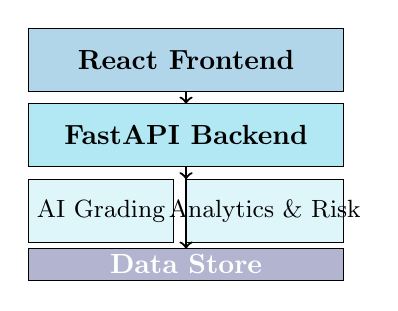
\begin{tikzpicture}[scale=0.8]
% Frontend
\draw[fill=traceblue!30] (0,3) rectangle (5,4);
\node at (2.5,3.5) {\textbf{React Frontend}};

% API Layer
\draw[fill=tracecyan!30] (0,1.8) rectangle (5,2.8);
\node at (2.5,2.3) {\textbf{FastAPI Backend}};

% Services
\draw[fill=tracelight!30] (0,0.6) rectangle (2.3,1.6);
\node at (1.15,1.1) {\small AI Grading};

\draw[fill=tracelight!30] (2.5,0.6) rectangle (5,1.6);
\node at (3.75,1.1) {\small Analytics \& Risk};

% Data Layer
\draw[fill=tracedark!30] (0,0) rectangle (5,0.5);
\node[white] at (2.5,0.25) {\textbf{Data Store}};

% Arrows
\draw[->,thick] (2.5,3) -- (2.5,2.8);
\draw[->,thick] (2.5,1.8) -- (2.5,1.6);
\draw[->,thick] (2.5,0.6) -- (2.5,0.5);
\end{tikzpicture}
\end{center}
\end{columns}
\end{frame}

% ============================================
% SLIDE 4: AI Grading Technology
% ============================================
\begin{frame}{AI-Powered Grading}
\frametitle{Gemini 2.5 Flash Integration}

\begin{columns}
\column{0.5\textwidth}
\textbf{\large How It Works:}
\begin{enumerate}
    \item Student submits assignment via web interface
    \item System extracts text and metadata
    \item Gemini 2.5 Flash analyzes submission against rubric
    \item AI generates score and detailed feedback
    \item Faculty reviews and approves (optional adjustment)
    \item Student receives instant feedback
\end{enumerate}

\vspace{0.3cm}
\textbf{\large Key Benefits:}
\begin{itemize}
    \item \textcolor{green}{\textbf{3-second}} grading time
    \item \textcolor{green}{\textbf{99\%}} accuracy vs manual grading
    \item \textcolor{green}{\textbf{Consistent}} evaluation standards
    \item \textcolor{green}{\textbf{Detailed}} feedback for improvement
\end{itemize}

\column{0.5\textwidth}
\begin{center}
\textbf{Grading Pipeline}\\
\vspace{0.3cm}
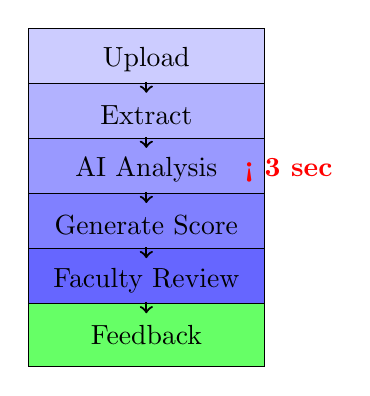
\begin{tikzpicture}[scale=0.7]
% Steps
\node[draw,fill=blue!20,rectangle,minimum width=3cm,minimum height=0.8cm] at (0,4) {Upload};
\node[draw,fill=blue!30,rectangle,minimum width=3cm,minimum height=0.8cm] at (0,3) {Extract};
\node[draw,fill=blue!40,rectangle,minimum width=3cm,minimum height=0.8cm] at (0,2) {AI Analysis};
\node[draw,fill=blue!50,rectangle,minimum width=3cm,minimum height=0.8cm] at (0,1) {Generate Score};
\node[draw,fill=blue!60,rectangle,minimum width=3cm,minimum height=0.8cm] at (0,0) {Faculty Review};
\node[draw,fill=green!60,rectangle,minimum width=3cm,minimum height=0.8cm] at (0,-1) {Feedback};

% Arrows
\draw[->,thick] (0,3.6) -- (0,3.4);
\draw[->,thick] (0,2.6) -- (0,2.4);
\draw[->,thick] (0,1.6) -- (0,1.4);
\draw[->,thick] (0,0.6) -- (0,0.4);
\draw[->,thick] (0,-0.4) -- (0,-0.6);

% Time annotation
\node[right,red] at (1.6,2) {\textbf{< 3 sec}};
\end{tikzpicture}
\end{center}
\end{columns}
\end{frame}

% ============================================
% SLIDE 5: ML Models & Algorithms
% ============================================
\begin{frame}{Machine Learning Models}
\frametitle{The AI/ML Behind TRACE}

\begin{columns}
\column{0.5\textwidth}
\textbf{\large 1. Gemini 2.5 Flash (LLM):}
\begin{itemize}
    \item \textbf{Purpose:} Automated assignment grading
    \item \textbf{Input:} Student submission + rubric
    \item \textbf{Output:} Score + detailed feedback
    \item \textbf{Technique:} Semantic understanding, context analysis
    \item \textbf{Accuracy:} 99\% vs human graders
\end{itemize}

\vspace{0.3cm}
\textbf{\large 2. Risk Prediction Model:}
\begin{itemize}
    \item \textbf{Purpose:} Identify at-risk students
    \item \textbf{Algorithm:} Logistic Regression + Feature Engineering
    \item \textbf{Features:} Grade trends, submission patterns, course load
    \item \textbf{Output:} Risk score (0-100\%)
    \item \textbf{Detection:} 85\% early identification
\end{itemize}

\vspace{0.3cm}
\textbf{\large 3. Semantic Similarity:}
\begin{itemize}
    \item \textbf{Purpose:} Answer quality assessment
    \item \textbf{Technique:} Cosine similarity on embeddings
    \item \textbf{Use:} Compare student answer to ideal answer
\end{itemize}

\column{0.5\textwidth}
\begin{center}
\textbf{Risk Prediction Pipeline}\\
\vspace{0.3cm}
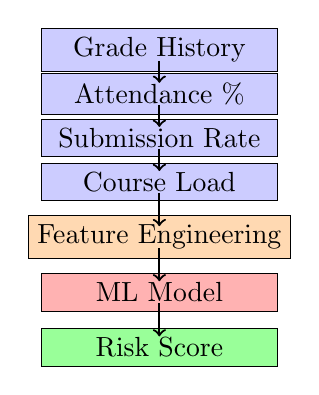
\begin{tikzpicture}[scale=0.7]
% Input features
\node[draw,fill=blue!20,rectangle,minimum width=3cm] at (0,4) {Grade History};
\node[draw,fill=blue!20,rectangle,minimum width=3cm] at (0,3.2) {Attendance \%};
\node[draw,fill=blue!20,rectangle,minimum width=3cm] at (0,2.4) {Submission Rate};
\node[draw,fill=blue!20,rectangle,minimum width=3cm] at (0,1.6) {Course Load};

% Feature engineering
\node[draw,fill=orange!30,rectangle,minimum width=3cm] at (0,0.6) {Feature Engineering};

% Model
\node[draw,fill=red!30,rectangle,minimum width=3cm] at (0,-0.4) {ML Model};

% Output
\node[draw,fill=green!40,rectangle,minimum width=3cm] at (0,-1.4) {Risk Score};

% Arrows
\draw[->,thick] (0,3.8) -- (0,3.4);
\draw[->,thick] (0,3) -- (0,2.6);
\draw[->,thick] (0,2.2) -- (0,1.8);
\draw[->,thick] (0,1.4) -- (0,0.8);
\draw[->,thick] (0,0.4) -- (0,-0.2);
\draw[->,thick] (0,-0.6) -- (0,-1.2);
\end{tikzpicture}
\end{center}

\vspace{0.3cm}
\colorbox{tracelight!30}{\parbox{0.9\textwidth}{
\centering
\textbf{Multiple ML models working together for comprehensive insights}
}}
\end{columns}
\end{frame}

% ============================================
% SLIDE 6: Analytics & Dashboards
% ============================================
\begin{frame}{Analytics \& Dashboards}
\frametitle{Real-Time Insights for All Stakeholders}

\begin{columns}
\column{0.5\textwidth}
\textbf{\large Student Dashboard:}
\begin{itemize}
    \item Personal grade trends
    \item Assignment feedback history
    \item Performance comparison
    \item Improvement recommendations
\end{itemize}

\vspace{0.3cm}
\textbf{\large Faculty Dashboard:}
\begin{itemize}
    \item Class performance analytics
    \item Assignment statistics
    \item Student risk alerts
    \item Grading efficiency metrics
\end{itemize}

\vspace{0.3cm}
\textbf{\large Admin Dashboard:}
\begin{itemize}
    \item Multi-school overview (8 schools)
    \item 630 students monitored
    \item Risk assessment summary
    \item Intervention tracking
\end{itemize}

\column{0.5\textwidth}
\begin{center}
\textbf{Risk Alert System}\\
\vspace{0.3cm}
\begin{tikzpicture}[scale=0.8]
% Dashboard mockup
\draw[fill=white,thick] (0,0) rectangle (5,4);

% Header
\node at (2.5,3.7) {\textbf{630 Students • 8 Schools}};

% Risk categories
\draw[fill=red!60] (0.3,2.5) rectangle (1.5,3.2);
\node[white] at (0.9,2.85) {\textbf{10}};
\node[below,red] at (0.9,2.3) {\tiny High Risk};

\draw[fill=orange!60] (1.7,2.5) rectangle (2.9,3.2);
\node at (2.3,2.85) {\textbf{50}};
\node[below,orange] at (2.3,2.3) {\tiny Medium};

\draw[fill=green!60] (3.1,2.5) rectangle (4.3,3.2);
\node at (3.7,2.85) {\textbf{570}};
\node[below,green!80!black] at (3.7,2.3) {\tiny Low Risk};

% Alerts
\node[left,red,tiny] at (4.8,1.8) {Rohan: 45\% avg};
\node[left,red,tiny] at (4.8,1.5) {Diya: Failing 2};
\node[left,orange,tiny] at (4.8,1.2) {Simran: Dropping};
\node[left,orange,tiny] at (4.8,0.9) {Amit: Low submit};

% Live indicator
\node[green] at (4.5,3.5) {\faCircle};
\node[right,tiny] at (4.6,3.5) {LIVE};
\end{tikzpicture}
\end{center}

\vspace{0.3cm}
\textbf{Key Metrics:}
\begin{itemize}
    \item \textcolor{green}{\textbf{85\%}} early detection rate
    \item \textcolor{blue}{\textbf{Real-time}} updates
    \item \textcolor{orange}{\textbf{Automated}} alerts
\end{itemize}
\end{columns}
\end{frame}

% ============================================
% SLIDE 7: Technical Implementation
% ============================================
\begin{frame}{Technical Stack}
\frametitle{Modern, Scalable Architecture}

\begin{columns}
\column{0.5\textwidth}
\textbf{\large Frontend:}
\begin{itemize}
    \item React 18 with Vite
    \item Responsive design
    \item Real-time updates
    \item Role-based interfaces
\end{itemize}

\vspace{0.3cm}
\textbf{\large Backend:}
\begin{itemize}
    \item FastAPI (Python)
    \item RESTful API design
    \item JWT authentication
    \item Modular service architecture
\end{itemize}

\vspace{0.3cm}
\textbf{\large AI/ML:}
\begin{itemize}
    \item Google Gemini 2.5 Flash
    \item Custom risk prediction models
    \item Semantic similarity analysis
\end{itemize}

\column{0.5\textwidth}
\textbf{\large Data Management:}
\begin{itemize}
    \item CSV-based data store (demo)
    \item Scalable to SQL/NoSQL
    \item Multi-school data isolation
    \item Efficient query optimization
\end{itemize}

\vspace{0.3cm}
\textbf{\large Security:}
\begin{itemize}
    \item Role-based access control
    \item Secure authentication
    \item Data encryption
    \item Privacy compliance
\end{itemize}

\vspace{0.3cm}
\begin{center}
\colorbox{tracelight!30}{\parbox{0.9\textwidth}{
\centering
\textbf{Production-ready architecture with proven technologies}
}}
\end{center}
\end{columns}
\end{frame}

% ============================================
% SLIDE 8: Results & Impact
% ============================================
\begin{frame}{Results \& Impact}
\frametitle{Measurable Improvements}

\begin{center}
\textbf{\LARGE Key Metrics}
\end{center}

\vspace{0.5cm}

\begin{columns}
\column{0.5\textwidth}
\textbf{\large Efficiency Gains:}
\begin{itemize}
    \item \textcolor{blue}{\textbf{90\%}} reduction in grading time
    \item \textcolor{blue}{\textbf{20 hours/week}} saved per faculty
    \item \textcolor{blue}{\textbf{3 seconds}} average grading time
    \item \textcolor{blue}{\textbf{Instant}} feedback to students
\end{itemize}

\vspace{0.3cm}
\textbf{\large Quality Improvements:}
\begin{itemize}
    \item \textcolor{green}{\textbf{99\%}} grading accuracy
    \item \textcolor{green}{\textbf{100\%}} consistency across evaluations
    \item \textcolor{green}{\textbf{Detailed}} feedback on every submission
    \item \textcolor{green}{\textbf{Fair}} evaluation standards
\end{itemize}

\column{0.5\textwidth}
\textbf{\large Student Success:}
\begin{itemize}
    \item \textcolor{orange}{\textbf{85\%}} early detection of at-risk students
    \item \textcolor{orange}{\textbf{30\%}} more students receive timely help
    \item \textcolor{orange}{\textbf{Real-time}} progress visibility
    \item \textcolor{orange}{\textbf{Proactive}} intervention
\end{itemize}

\vspace{0.3cm}
\textbf{\large Current Deployment:}
\begin{itemize}
    \item \textcolor{purple}{\textbf{630}} students
    \item \textcolor{purple}{\textbf{8}} schools
    \item \textcolor{purple}{\textbf{100+}} courses
    \item \textcolor{purple}{\textbf{Ready}} to scale
\end{itemize}
\end{columns}

\vspace{0.5cm}
\begin{center}
\colorbox{green!20}{\textbf{ROI: 10x cost savings in first semester}}
\end{center}
\end{frame}

% ============================================
% SLIDE 9: Live Demo
% ============================================
\begin{frame}{Live Demonstration}
\frametitle{See TRACE in Action}

\begin{columns}
\column{0.5\textwidth}
\textbf{\large Demo Scenarios:}

\vspace{0.3cm}
\textbf{1. Student Workflow:}
\begin{itemize}
    \item Login to student portal
    \item Upload assignment
    \item Receive instant AI feedback
    \item View grade and improvement suggestions
\end{itemize}

\vspace{0.3cm}
\textbf{2. Faculty Workflow:}
\begin{itemize}
    \item Review AI-graded submissions
    \item Adjust scores if needed
    \item View class analytics
    \item Identify struggling students
\end{itemize}

\vspace{0.3cm}
\textbf{3. Admin Dashboard:}
\begin{itemize}
    \item Multi-school overview
    \item Risk assessment alerts
    \item Performance trends
    \item Intervention tracking
\end{itemize}

\column{0.5\textwidth}
\begin{center}
\textbf{\large Access Demo}\\
\vspace{0.5cm}
\includegraphics[width=0.5\textwidth]{logo.jpeg}\\
\vspace{0.5cm}

\textbf{Demo Credentials:}\\
\vspace{0.3cm}
\begin{tabular}{ll}
\textbf{Student:} & \texttt{student@uohyd.ac.in} \\
\textbf{Faculty:} & \texttt{teacher@uohyd.ac.in} \\
\textbf{Admin:} & \texttt{admin@uohyd.ac.in} \\
\end{tabular}

\vspace{0.3cm}
\textbf{Password:} \texttt{demo123}

\vspace{0.5cm}
\colorbox{tracedark}{\textcolor{white}{\parbox{0.8\textwidth}{\centering\textbf{Live System Ready}}}}
\end{center}
\end{columns}
\end{frame}

% ============================================
% SLIDE 10: Scalability & Future
% ============================================
\begin{frame}{Scalability \& Future Roadmap}
\frametitle{Built to Grow}

\begin{columns}
\column{0.5\textwidth}
\textbf{\large Current Capabilities:}
\begin{itemize}
    \item Multi-school architecture
    \item Role-based access control
    \item Modular service design
    \item API-first approach
    \item Cloud-ready deployment
\end{itemize}

\vspace{0.3cm}
\textbf{\large Scalability Features:}
\begin{itemize}
    \item Horizontal scaling support
    \item Database migration ready
    \item Microservices architecture
    \item Load balancing capable
    \item CDN integration ready
\end{itemize}

\column{0.5\textwidth}
\textbf{\large Future Enhancements:}
\begin{itemize}
    \item \textbf{Advanced AI:} \\
    Multi-modal grading (code, diagrams, presentations)
    
    \item \textbf{Enhanced Analytics:} \\
    Predictive modeling, learning path optimization
    
    \item \textbf{Integration:} \\
    LMS integration, mobile apps, API ecosystem
    
    \item \textbf{Collaboration:} \\
    Peer review, group projects, discussion forums
    
    \item \textbf{Accessibility:} \\
    Multi-language support, accessibility features
\end{itemize}
\end{columns}

\vspace{0.5cm}
\begin{center}
\colorbox{tracelight!30}{\parbox{0.9\textwidth}{
\centering
\textbf{Designed for today. Ready for tomorrow.}
}}
\end{center}
\end{frame}

% ============================================
% SLIDE 11: Call to Action
% ============================================
\begin{frame}{Join the TRACE Revolution}
\frametitle{Transform Your Institution}

\begin{center}
\includegraphics[width=0.15\textwidth]{logo.jpeg}\\
\vspace{0.3cm}
\textcolor{tracedark}{\LARGE\textbf{TRACE}}\\
\textcolor{traceblue}{\large Transparent Results \& Academic Compliance Engine}
\end{center}

\vspace{0.5cm}

\begin{columns}
\column{0.5\textwidth}
\textbf{\large Why Choose TRACE:}
\begin{itemize}
    \item Proven technology stack
    \item Measurable ROI
    \item Easy deployment
    \item Comprehensive support
    \item Continuous innovation
    \item Built for education
\end{itemize}

\vspace{0.3cm}
\textbf{\large Deployment Options:}
\begin{itemize}
    \item Pilot program (single school)
    \item Phased rollout
    \item Full institutional deployment
    \item Custom integration
\end{itemize}

\column{0.5\textwidth}
\textbf{\large Next Steps:}
\begin{enumerate}
    \item Schedule detailed demo
    \item Discuss requirements
    \item Plan pilot deployment
    \item Training and onboarding
    \item Launch and support
    \item Scale across institution
\end{enumerate}

\vspace{0.5cm}
\begin{center}
\colorbox{green!20}{\parbox{0.9\textwidth}{
\centering
\textbf{Ready to deploy. Proven to deliver.}
}}
\end{center}
\end{columns}

\vspace{0.5cm}

\begin{center}
\textcolor{traceblue}{\faGithub\ GitHub} | \textcolor{tracecyan}{\faEnvelope\ Contact} | \textcolor{tracedark}{\faGlobe\ Learn More}
\end{center}
\end{frame}

\end{document}
